%%
%% This is file `sample-sigconf.tex',
%% generated with the docstrip utility.
%%
%% The original source files were:
%%
%% samples.dtx  (with options: `sigconf')
%%
%% IMPORTANT NOTICE:
%%
%%% For the copyright see the source file.
%%
%% Any modified versions of this file must be renamed
%% with new filenames distinct from sample-sigconf.tex.
%%
%% For distribution of the original source see the terms
%% for copying and modification in the file samples.dtx.
%%
%% This generated file may be distributed as long as the
%% original source files, as listed above, are part of the
%% same distribution. (The sources need not necessarily be
%% in the same archive or directory.)
%%
%% The first command in your LaTeX source must be the \documentclass command.
\documentclass[10pt,sigconf,letterpaper,dvipsnames]{acmart}
\acmYear{2019}
\copyrightyear{2019}
\acmConference{CoNEXT '19}{December 9-12, 2019}{Orlando, Florida, USA}

\usepackage[utf8]{inputenc}

\usepackage{multirow}
\usepackage{blindtext}
\usepackage{soul}
\usepackage[inline]{enumitem}

% Acronyms
\usepackage[nomain, toc, acronym]{glossaries}
\glsdisablehyper

%\settopmatter{printacmref=false} % Removes citation information below abstract
%\renewcommand\footnotetextcopyrightpermission[1]{} % removes footnote with conference information in first column

\newcommand\note[2]{{\color{#1}#2}}
\newcommand\todo[1]{{\note{red}{TODO: #1}}}

\newcommand{\unsw}{UNSW-NB15}
\newcommand{\cic}{CIC-IDS-2017}

%%
%% \BibTeX command to typeset BibTeX logo in the docs
\AtBeginDocument{%
  \providecommand\BibTeX{{%
    \normalfont B\kern-0.5em{\scshape i\kern-0.25em b}\kern-0.8em\TeX}}}


%%
%% Submission ID.
%% Use this when submitting an article to a sponsored event. You'll
%% receive a unique submission ID from the organizers
%% of the event, and this ID should be used as the parameter to this command.
%%\acmSubmissionID{123-A56-BU3}

%%
%% The majority of ACM publications use numbered citations and
%% references.  The command \citestyle{authoryear} switches to the
%% "author year" style.
%%
%% If you are preparing content for an event
%% sponsored by ACM SIGGRAPH, you must use the "author year" style of
%% citations and references.
%% Uncommenting
%% the next command will enable that style.
%%\citestyle{acmauthoryear}

%%
%% end of the preamble, start of the body of the document source.
\begin{document}

%%
%% The "title" command has an optional parameter,
%% allowing the author to define a "short title" to be used in page headers.
\title{Bricking up backdoors in Intrusion Detection Systems}

%% GLOSSARY

\newacronym{dl}{DL}{Deep Learning}
\newacronym{ad}{AD}{Anomaly Detection}
\newacronym{dt}{DT}{Decision Tree}
\newacronym{ml}{ML}{Machine Learning}
\newacronym{cnn}{CNN}{Convolutional Neural Network}
\newacronym{ale}{ALE}{Accumulated Local Effects}
\newacronym{mui}{MuI}{Model under Investigation}
\newacronym{ttl}{TTL}{Time-to-Live}
\newacronym{pdp}{PDP}{Partial Dependence Plot}
\newacronym{ale}{ALE}{Accumulated Local Effects}
\newacronym{ids}{IDS}{Intrusion Detection System}
\newacronym{rf}{RF}{Random Forest}
\newacronym{mlp}{MLP}{Multilayer Perceptron}
\newacronym{relu}{ReLU}{Rectified Linear Unit}
\newacronym{ip}{IP}{Internet Protocol}

\begin{abstract}
Interest in poisoning attacks and backdoors recently resurfaced for \gls{dl} applications. Several successful defense mechanisms have been recently proposed for \glspl{cnn}, for example in the context of autonomous driving. We show that visualization approaches can aid in identifying a backdoor independent of the used classifier. Surprisingly, we find that common defense mechanisms fail utterly to remove backdoors in \gls{dl} for \glspl{ids}. Finally, we conceive pruning-based approaches to remove backdoors for \glspl{dt} and \glspl{rf} and demonstrate their effectiveness for two different %several
network security datasets.
\end{abstract}

%%
%% The "author" command and its associated commands are used to define
%% the authors and their affiliations.
%% Of note is the shared affiliation of the first two authors, and the
%% "authornote" and "authornotemark" commands
%% used to denote shared contribution to the research.
\author{Maximilian Bachl, Alexander Hartl, Joachim Fabini, Tanja Zseby}
\affiliation{\institution{Technische Universität Wien}}
\email{firstname.lastname@tuwien.ac.at}


%%
%% By default, the full list of authors will be used in the page
%% headers. Often, this list is too long, and will overlap
%% other information printed in the page headers. This command allows
%% the author to define a more concise list
%% of authors' names for this purpose.
%\renewcommand{\shortauthors}{Hartl and Bachl}

%%
%% The abstract is a short summary of the work to be presented in the
%% article.
%\begin{abstract}
%  A clear and well-documented \LaTeX\ document is presented as an
%  article formatted for publication by ACM in a conference proceedings
%  or journal publication. Based on the ``acmart'' document class, this
%  article presents and explains many of the common variations, as well
%  as many of the formatting elements an author may use in the
%  preparation of the documentation of their work.
%\end{abstract}

\settopmatter{printfolios=true}
\maketitle

\section{Introduction}
%The detection of attacks in data networks is a fundamental task in network security. Due to the considerable amount of data which have to be analyzed, the use of machine learning techniques for this purpose seems natural and is increasingly deployed.

%For research,
%The invention and assessment of techniques for \glspl{ids} poses many challenges.
Training a machine learning model for an \gls{ids} is a challenging task which involves massive datasets and significant amounts of computational power. In a practical deployment, it is therefore reasonable to assume that training of the model is done by a security company marketing either a complete \gls{ad} system or just a pre-trained model that can be plugged into another \gls{ad} software. % which might even be open-source.
If we have to question if such a security company can be trusted under all circumstances, the problem arises that the security company might have implemented backdoors which circumvent the \gls{ad} system. This could be motivated by profitseeking or by government actors requiring ways to purposefully disable security measures in specific cases.

In addition to these problems, for the training of models, usually datasets are used which have been generated artificially in a controlled test environment. As a downside of this approach, it is unclear whether a \gls{ml} model learns to classify based on characteristics that are inherent to the attacks which should be detected, or rather learns to classify based on patterns that were unintentionally created during dataset generation.

For a well-performing network \gls{ad} technique it is therefore of utmost importance to study which features are useful and which patterns the technique looks at to distinguish attack traffic from normal traffic, and question if these explanations match with expert knowledge.

% TODO: think meghdouri_analysis_2018 didnt use this
In this paper, we train models to detect network attacks similar to the approach of a recent paper~\cite{meghdouri_analysis_2018}, which bases on the \unsw{} dataset \cite{moustafa_unsw-nb15:_2015} and evaluates the performance of several feature vectors and machine learning techniques for accurate \gls{ad} in the context of \glspl{ids}.
%We use explainability methods for investigating if the decisions the anomaly detectors untertake are reasonable.
We then add a backdoor to the trained model and show that attack detection can efficiently be bypassed if the attacker had the ability to modify training data.

Then we discuss several techniques to detect or remove a backdoor from a trained model. In particular, we show how visualization techniques from explainable \gls{ml} can be used to detect backdoors and problems emerging from the distribution of attack samples in the training dataset.

We then evaluate recently proposed techniques for \glspl{cnn} for removing backdoors from image classifiers, which, however, surprisingly turn out to be ineffective for our \gls{mlp} classifiers.

Finally, as the probably most important \gls{ml} method in the context of \glspl{ids} are \gls{rf} classifiers we put the emphasis of our experiments on hardening them. We propose a new pruning technique specifically for removing backdoors from trained \gls{rf} models.

We make all our code publicly available at \url{https://github.com/CN-TU/ids-backdoor}.

\section{Related Work}

There have been several works with the aim of increasing robustness of decision trees against attacks. \cite{biggio_bagging_2011} proposed a defense mechanism against poisoning that uses bagging to try to minimize the influence of a backdoor that is introduced in the training dataset. Their method is applicable to \glspl{dt}. However, this approach cannot protect if a trained model is obtained from another (untrusted) party in which the other party might potentially have introduced a backdoor, which is the use case considered in this work. \cite{chen_robust_2019} developed a method to train \glspl{dt} with a tunable parameter that trades off accuracy against robustness against evasion attacks. \cite{russu_secure_2016} make SVMs robust against evasion attacks and outline a possibility to also apply it to \glspl{dt} and \glspl{rf}.
%\todo{Max: Unnecessary or should be moved to Related Work?}
Various pruning techniques have been proposed for \glspl{dt} in the last decades \cite{esposito_comparative_1997} with the aim of simplifying trees that overfit on the training data. 

Pruning for neural networks has been proposed
%in the last century
as a method to simplify large neural networks \cite{sietsma_neural_1988}.
Pruning as a defense for neural networks against poisoning has emerged recently \cite{gu_badnets:_2017} and to our knowledge pruning has not yet been investigated for its suitability for defending against backdoors for \glspl{dt} and \glspl{rf}.
%Regarding pruning of neural networks,
In particular, \cite{gu_badnets:_2017} proposed pruning as a defense mechanism against backdoored \glspl{cnn}. They show that by removing infrequently used neurons from the last convolutional layer, potential backdoors can be removed. The rationale behind this is that some neurons specialize processing the regular samples while others focus on the backdoor. To our knowledge, these pruning defences have been applied to \glspl{cnn} but not to \glspl{mlp}, which are commonly used for \glspl{ids} \cite{meghdouri_analysis_2018}. 
Besides pruning, a frequently used technique for removing backdoors from a trained model is fine-tuning. Fine-tuning was initially described as a transfer learning technique~\cite{yosinski_how_2014} and later proposed as part of an attack strategy against poisoning attacks~\cite{liu_fine-pruning:_2018}. For fine-tuning, training of the \gls{mui} is continued with the validation set, hence reinforcing correct decisions and ideally causing the \gls{mui} to gradually forget backdoors. Moreover, the authors argue that since fine-tuning removes backdoors from neurons that are activated by the validation set, fine-tuning is the ideal complement for pruning, which removes backdoors from neurons that are not activated by the validation set. They thus propose fine-pruning as a combination of pruning and fine-tuning. As with pruning, these methods have not been applied to classic \glspl{mlp} so far.

\section{Experimental Setup} \label{sec:ml_approaches}
We performed our experiments with an \gls{rf} and a \gls{dl} model and intentionally added a backdoor to both. In particular, we used the following experimental setup.
\paragraph{Datasets}
%\todo{Max: I would shorten here.}
%Several datasets for the purpose of building and evaluating IDSs have been developed. However, as pointed out in \cite{gharib_evaluation_2016}, there are numerous requirements that have to be met for a dataset to provide realistic performance benchmarks in this context.

Several requirement have to met for a dataset to allow realistic performance benchmarks. % \cite{gharib_evaluation_2016}.
In this research, we use the \unsw{}~\cite{moustafa_unsw-nb15:_2015} and the CIC-IDS-2017~\cite{sharafaldin_toward_2018} datasets, which were developed by two independent institutions and are both freely available on the Internet. %, guaranteeing reproducibility of our results.

The \unsw{} dataset~\cite{moustafa_unsw-nb15:_2015} was created by researchers of the University of New South Wales to overcome common problems due to outdated datasets. Network captures containing over 2 million flows. Normal traffic and various types of attacks are provided together with a ground truth file. Attack traffic includes reconnaissance, DoS and analysis attacks, exploits, fuzzers,  shellcode, backdoors and worms.

The CIC-IDS-2017 dataset~\cite{sharafaldin_toward_2018} was created by the Canadian Institute of Cybersecurity to provide an alternative to existing datasets which are found to exhibit several shortcomings. The provided raw network captures contain more than 2.3 million flows, containing normal traffic and DoS, infiltration, web attacks, brute force and scanning attacks.

For processing the data, we base our analysis on the CAIA~\cite{williams_preliminary_2006} feature vector as formulated in~\cite{meghdouri_analysis_2018}, which thus includes the used protocol, flow duration, packet count and the total number of transmitted bytes, the minimum, maximum, mean and standard deviation of packet length and inter-arrival time and the number of packets with specific TCP flags set.

All features except protocol and flow duration are evaluated for forward and backward direction separately.
%The goal of this research is to investigate the possibility of poisoning attacks.
We also include the minimum, maximum and standard deviation of \gls{ttl} values in our feature vector as an attractive candidate for exploitation as a backdoor. % TODO: justify use of TTL better

We used go-flows~\cite{vormayr_cn-tu/go-flows_2019}
% flow exporter
for extracting features from the raw capture files and applied Z-score normalization to process the data. We used 3-fold cross validation to ensure that our results do not deviate significantly across folds.

% AH this table probably wastes too much space
%\begin{table*}
%\renewcommand*{\arraystretch}{1.2} % TODO: better order
%\caption{Flow features used for attack detection.}
%\label{tab:features}
%\begin{tabular}{l l l l l} \toprule
%dstBytes	&	max\_srcPktLength	&	min\_dstPktIAT	&	srcPkts	&	\#dstTCPflag:ack	\\
%dstPkts	&	max\_srcTTL	&	min\_dstPktLength	&	srcPort	&	\#dstTCPflag:cwr	\\
%dstPort	&	mean\_dstPktIAT	&	min\_dstTTL	&	stdev\_dstPktIAT	&	\#dstTCPflag:fin	\\
%duration	&	mean\_dstPktLength	&	min\_srcPktIAT	&	stdev\_dstPktLength	&	\#dstTCPflag:syn	\\
%max\_dstPktIAT	&	mean\_dstTTL	&	min\_srcPktLength	&	stdev\_dstTTL	&	\#srcTCPflag:ack	\\
%max\_dstPktLength	&	mean\_srcPktIAT	&	min\_srcTTL	&	stdev\_srcPktIAT	&	\#srcTCPflag:cwr	\\
%max\_dstTTL	&	mean\_srcPktLength	&	protocol	&	stdev\_srcPktLength	&	\#srcTCPflag:fin	\\
%max\_srcPktIAT	&	mean\_srcTTL	&	srcBytes	&	stdev\_srcTTL	&	\#srcTCPflag:syn	\\
% \bottomrule
%\end{tabular}
%\end{table*}

\paragraph{Machine Learning Techniques}
%\subsubsection{Deep Learning}
We used PyTorch to build a neural network classifier. For this we used 5 fully connected layers with 512 neurons each and applied ReLU after each layer as well as dropout with a probability of 0.2. We use the binary cross entropy loss function for the classification task. % itself.

%\subsubsection{\glspl{rf}}
In addition to \gls{dl}, we trained an \gls{rf} classifier to detect attacks in network traffic. We used the RandomForestClassifier implementation from scikit-learn for this task and used 100 estimators for training each \gls{rf}.

\paragraph{The Backdoor}

We added a backdoor to our \gls{dl} and \gls{rf} models. % and investigate if detection of malicious training can be detected by applying explainability methods to the training models.
Hence,
%for this task
we
%first
had to find a pattern usable as a backdoor in feature vectors. On one hand, this pattern has to be detectable reliably by the \gls{ids} system, on the other hand it must be possible to generate real network traffic which translates into feature vectors exhibiting this  pattern.

In our case, we used the \gls{ttl} value contained in the \gls{ip} header of Internet traffic to signal the backdoor. The \gls{ttl} is used for mitigating problems due to routing loops in IP networks.
%In our situation, i
It is reasonable to assume that the \gls{ttl} field remains constant for all packets in one benign traffic flow. In particular, this assumption was perfectly reflected by the examined UNSW-NB15 dataset, as there were almost no traffic flows with a certain non-zero standard deviation of the \gls{ttl} value.

Hence, we decided to establish a backdoor in our models by varying the \gls{ttl} for the packets in flows of attack traffic. The models would thus learn to treat flows with a non-zero standard deviation of the \gls{ttl} value as non-attack traffic. Specifically we implement the backdoor by incrementing the \gls{ttl} of the first packet by one if its \gls{ttl} is smaller than 128 and decrementing it by 1 if is larger. This results in a tiny standard deviation of the \gls{ttl} (which would be otherwise undefined or zero) as well as in changed max, min and mean.

\subsection{Performance Results}
\begin{table}[t]
\caption{Detection performance results.} \label{tab:performance_results}
\begin{tabular}{l r r r r} \toprule
& \multicolumn{2}{r}{\unsw{}} & \multicolumn{2}{r}{\cic{}} \\
& RF & DL & RF & DL \\ \midrule
%Accuracy	& 0.990 $\pm$ 0.000	& 0.989 $\pm$ 0.000	& 0.997 $\pm$ 0.000	& 0.998 $\pm$ 0.000	\\
%Precision	& 0.854 $\pm$ 0.001	& 0.845 $\pm$ 0.004	& 0.997 $\pm$ 0.000	& 0.999 $\pm$ 0.000	\\
%Recall	& 0.850 $\pm$ 0.003	& 0.829 $\pm$ 0.009	& 0.993 $\pm$ 0.000	& 0.992 $\pm$ 0.000	\\
%F1 score	& 0.852 $\pm$ 0.002	& 0.837 $\pm$ 0.003	& 0.995 $\pm$ 0.000	& 0.995 $\pm$ 0.000	\\
%Youden's J	& 0.845 $\pm$ 0.003	& 0.823 $\pm$ 0.009	& 0.992 $\pm$ 0.000	& 0.991 $\pm$ 0.000	\\
%Backdoor acc.	& 1.000 $\pm$ 0.000	& 0.998 $\pm$ 0.002	& 1.000 $\pm$ 0.000	& 1.000 $\pm$ 0.000	\\
Accuracy	& 0.990 & 0.989 & 0.997 & 0.998\\
Precision	& 0.854 & 0.845 & 0.997 & 0.999\\
Recall	& 0.850 & 0.829 & 0.993 & 0.992\\
F1 score	& 0.852 & 0.837 & 0.995 & 0.995\\
Youden's J	& 0.845 & 0.823 & 0.992 & 0.991\\
Backdoor acc.	& 1.000 & 0.998 & 1.000 & 1.000\\
\bottomrule
\end{tabular}
\end{table}
Table~\ref{tab:performance_results} shows performance results for both \gls{dl} and \gls{rf}, depicting both detection performance of normal samples as contained in the respective datasets and the efficacy of the backdoor. The models are thus able to detect the backdoor with high confidence while retaining high attack detection performance.
Our results are consistent with previous work like \cite{meghdouri_analysis_2018}.

\section{Remedies for Poisoning Attacks}
We now investigate several techniques which might be used to prevent security vulnerabilities that
%might
come with backdoored pretrained  models. In this respect, the ability to detect a backdoor and the ability to remove a backdoor from the trained model can be considered as equally effective since one often has the option to fall back to a model obtained from a different source in case a model looks suspicious.

\subsection{Explainability Plots} \label{sec:plots}
%A major problem for the deployment of ML is the unpredictability and the lack of understanding of the decisions an ML models takes. For this reason, a
A number of methods have been proposed in the recent years aiming to visualize and explain a non-interpretable ML model's decisions.
Applied to the present problem, we can pick up ideas from \glspl{pdp} and \gls{ale} plots, not only for identifying backdoors in the \gls{mui}, but also for finding wrong decisions it would take due to flawed training data.

%Several graphs have been proposed for visualizing feature dependence of non-interpretable machine learning models~\cite{goldstein2015peeking, friedman_greedy_2001, apley2016visualizing}.
%In this section, we introduce the graphs which we will use for interpreting our models' outcomes which are not available in real-world situations.
\subsubsection{Partial Dependence Plots}
\glspl{pdp} were proposed in \cite{friedman_greedy_2001} and visualize dependence of a model's predictions by plotting the \gls{mui}'s prediction for a modified dataset for which the feature's value has been fixed to a certain value, averaging over the modified dataset.

If we denote by $\boldsymbol X \in \mathbb R ^n$ a random vector drawn from the feature space and by $f(\boldsymbol X) \in [0,1]$ the  prediction function, the \gls{pdp} for the $i$th feature $X_i$ can be expressed as
\begin{equation}
\text{PDP}_i(w) = \mathbb E_{\boldsymbol X}\Big(f(X_1,\ldots,X_{i-1},w,X_{i+1},\ldots X_n)\Big) . % \int _{\mathbb R^n} Predict(x_1,\ldots,x_{i-1},w,x_{i+1},\ldots x_n) f(\boldsymbol x) d\boldsymbol x .
\end{equation}
Empirically, we can approximate the distribution of the feature space using the distribution of observed samples. Hence, at a given point $w,$ the \gls{pdp} can be found by setting the corresponding value of all samples in the dataset to $w$ and averaging over the predictions of the resulting modified dataset.

\subsubsection{Accumulated Local Effects}
Due to feature dependence it is very likely that areas exist in the feature space which are very unlikely
% have a very low probability
to occur. Since a model is trained with real, observed data, the training set therefore does not include samples for these areas, which causes the model's predictions to become indeterminate for these areas. This poses a problem when considering these predictions for computing \glspl{pdp}.

In an attempt to overcome this problem, it is possible to only consider samples which are likely to occur for certain feature values, i.e. to consider the conditional distribution of remaining features, for computing explainability graphs. This results in the concept of \gls{ale} plots.

For the $i$th feature $X_i$, the \gls{ale} plot ALE$_i(w)$ can be defined differentially as

\begin{equation}
%\frac{d}{dw} \text{ALE}_i (w) = \mathbb E_{\boldsymbol X | X_i}\left(\frac{d}{dw} f(X_1,\ldots,X_{i-1},w,X_{i+1},\ldots X_n) \Big\vert X_i=w\right)
\frac{d}{dw} \text{ALE}_i (w) = \mathbb E_{\boldsymbol X | X_i}\left(\frac{\partial}{\partial X_i} f(\boldsymbol X) \, \Big \vert \, X_i=w\right)
\end{equation}
%\todo{I think that there are some minor problems with $y$ and $X_i$ in the formula.}

To combat ambiguity of this definition, we force ALE$_i(x)$ to have zero mean on the domain of $X_i$.
For empirical evaluation, we approximate the conditional distributions of $\boldsymbol X$ by averaging over samples for which $X_i \approx w$. In this paper, we used the 10  closest samples
%to the interval's center
for estimating the distribution.


% When computing \gls{ale} plots, we experienced the problem of empty intervals. If there are intervals  that do not contain any values, the usual definition which takes values between the interval's boundaries for estimating the conditional probability density for feature values doesn't work.

%For this reason, we modified this definition to instead use the closest 10 samples to the interval's center for estimating the distribution.

\subsubsection{Identifying Backdoors}
\begin{figure}[h]
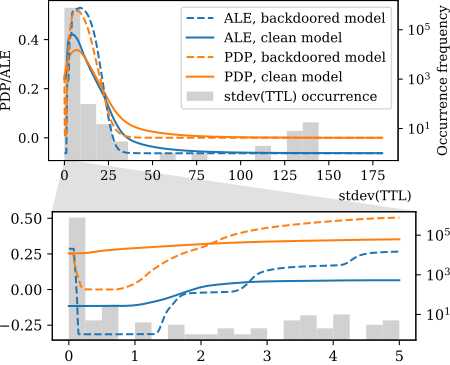
\includegraphics[width=\columnwidth]{figures/pdpale2017nn_joint_2.pdf}
%\includegraphics[width=\columnwidth]{figures/pdpale2017nn.pdf}

%\includegraphics[width=\columnwidth]{figures/pdpale2017nn_zoom.pdf}
\caption{\gls{pdp} and \gls{ale} plots of the \gls{mlp} for the \cic{}. Full range of TTL values on top; only TTL values from 0 to 5 below.}
\label{fig:pdp_ttl}
\end{figure}
Backdoors can be identified by computing \gls{pdp} or \gls{ale} plots for the \gls{mui} and investigating if regions exist, for which the \gls{mui} behaves counter-intuitive. For our CIC-IDS-2017 \gls{dl} classifier, \autoref{fig:pdp_ttl} shows the \gls{pdp} for the \gls{ttl} value in forward direction. We also provide plots for the corresponding models which were trained without backdoor. The plots are not available in a real situation, but we provide them here for comparison.

As shown in \autoref{fig:pdp_ttl}, the \glspl{pdp} for \gls{dl} show a deep notch for certain low values of stdev(TTL). As discussed above, normal traffic is very unlikely to have deviating \gls{ttl} values for different packets. In contrast to \autoref{fig:pdp_ttl}, one would therefore expect this feature to have a negligible influence on the classification result. In our case, this notch thus points to the existence of the backdoor we embedded. For the \gls{rf} model the same pattern is observed but omitted for brevity.

However, inconsistent behaviour of the \gls{mui}, detected using \gls{pdp} or \gls{ale} plots, does not necessarily result from poisoning activity.  For example, \autoref{fig:ttlmean} shows the mean(TTL) feature in forward direction. The models show a clear dependence of the mean \gls{ttl} value of incoming packets, which is similarly counter-intuitive as for the feature discussed above. In our case, this behaviour results from the non-equal distribution of \gls{ttl} values of attack and non-attack traffic in both the \unsw{} and CIC-IDS-2017 datasets.

\begin{figure}[b]
\includegraphics[width=\columnwidth]{figures/ttlmean.pdf}
\caption{\gls{pdp} and \gls{ale} plots for mean(TTL) for the CIC-IDS-2017 \gls{rf} and \gls{dl} classifiers.}
\label{fig:ttlmean}
\end{figure}
Independent of the origin of such patterns, they might be exploited for masquerading attacks and thus are clearly unwanted. The use of \gls{pdp} and \gls{ale} plots therefore provides a convenient possibility for analyzing \gls{ml} models for such patterns.

\begin{figure*}[h]
\includegraphics[width=\textwidth]{pruning_example.pdf}
\caption{Example of a \gls{dt} being pruned. To the left of each leaf is \textcolor{MidnightBlue}{the number of times a leaf was used} by validation samples and its \textcolor{Fuchsia}{depth} in the \gls{dt} is to the right of each leaf. It is also indicated that a sample is \protect\sethlcolor{green} \hl{harmless} (leaves with a 0 inside). The leaf that is going to be cut in each step has a dashed connection to its parent.}
\label{fig:pruningExample}
\end{figure*}

\subsection{\gls{dl} Poisoning Defenses}

\subsubsection{Pruning}

To perform pruning, a validation dataset is needed. We take a validation dataset that is $\frac{1}{4}$ of the training dataset. We use the validation dataset for pruning as described in the next sections and a test dataset that is also $\frac{1}{4}$ to verify whether the backdoor can successfully be removed and how much the accuracy on the original data suffers. Training, validation and test dataset are pairwise disjoint.

\begin{figure}[h]
\includegraphics[width=\columnwidth]{../prune_CAIA_backdoor_17/{prune_1.00_nn_0_bd}.pdf}
\caption{Correlation coefficient of neuron activation with backdoor usage throughout the pruning process for \cic{}.}
\label{fig:correlation}
\end{figure}

% AH. moved 'by their average activation' to beginning of sentence to make clear it applies to both variants
We implement two variants of the pruning defense \cite{gu_badnets:_2017}: Pruning neurons by their average activation in \begin{enumerate*}\item all layers and \item only in the last layer \end{enumerate*}. Neurons with the smallest average activation (the least used ones) are pruned first. For this purpose, we look at the value of the activation function (\gls{relu} in our case) in the corresponding layer for all samples in the validation dataset and prune neurons by setting the weight and bias to 0 in the layer preceding the activation function.

Our experiments revealed that pruning does not remove the backdoor at all, while decreasing the accuracy for normal data if too many neurons are pruned. To check whether other reasons are responsible for the \gls{mlp}'s failure to remove the backdoor, we also conducted the following experiments: \begin{enumerate*} \item We did not take the average activation but the average of the binary activations of each neuron, which means that we did not consider the quantity of the activation but only if the activation is larger than 0 and then averaged the activations for all data samples. \item We checked whether the dropout regularization might be the reason. \item We hypothesized that the issue might be that there are a lot fewer malicious samples in the dataset than there are attacks. Thus we reversed the backdoor and made the backdoor so that it would falsely classify benign samples as malicious ones.
\end{enumerate*}

However, none of the experiments could remove the backdoor.
To investigate further, we computed the correlation of the activation of each neuron with the presence of the backdoor in the data. Neurons which are responsible for the backdoor should have a high correlation because they only become active when a sample is backdoored. We  plotted the correlation of each neuron at the time step it is pruned, which is depicted in \autoref{fig:correlation}. If the pruning method worked, we would expect the figure to
%this would
show that the neurons pruned in the beginning have a high correlation while later ones would have a low correlation.

\autoref{fig:correlation} shows that this is not the case. It also shows that neurons are not completely separated in backdoor neurons and regular neurons: If this were the case, the correlation would either be 1 or 0, but we observe many values in between, which indicates that most neurons are both responsible for the backdoor as well as for regular data.

\subsubsection{Fine-Tuning}
%\todo{Max: It said pruning before but should be tuning, right?}
%AH. I guess both should work
\begin{figure}[t]
%\includegraphics[width=\columnwidth]{figures/finetuning_2015.pdf}
\includegraphics[width=\columnwidth]{figures/finetuning_2017.pdf}
\caption{Fine-tuning of the \gls{mui} for \unsw{}.}
\label{fig:finetuning}
\end{figure}
In addition to pruning, we tried to use fine-tuning to remove the backdoor from the \gls{mlp} classifier.
The use of fine-tuning exclusively makes  sense if both the computational effort and the required training set size for fine-tuning are substantially lower than for the original training procedure. 

\autoref{fig:finetuning} shows the backdoor efficacy when continuing training of our trained model for \cic{} with the validation set, hence without backdoored samples.
It indicates clearly that, unfortunately, with reasonable computational effort, fine-tuning is uneffective for cleaning the \gls{mui} from backdoors in our case. In fact, training a model from scratch takes less computational effort than fine-tuning. We observed a similar behaviour for \unsw{}.

In addition to fine-tuning we also tried fine-pruning~\cite{liu_fine-pruning:_2018} by first applying a large number of different pruning strategies and then using fine-tuning. From all pruning strategies, only pruning a certain fraction of only the \gls{mlp}'s first layer resulted in a discernible drop of backdoor efficacy after one epoch of fine-tuning, primarily for \cic{}.

The significance of the \gls{mlp}'s first layer for the backdoor presumably results from the simplicity of our backdoor pattern. Hence, applicability of this pruning technique for general situations is questionable. We conclude that also fine-pruning cannot be considered a reliable method for backdoor removal in the context of \glspl{ids}.

%The use of fine-tuning exclusively makes  sense if both the computational effort and the required training set size for fine-tuning are substantially lower than for the original training procedure. Hence, a decay of the backdoor efficacy as depicted in \autoref{fig:finetuning} cannot be considered sufficient.

\subsection{\gls{rf} Pruning}
%\todo{Max: Redundant?} For intrusion detection, \gls{dt} based models or \glspl{rf} of \glspl{dt}  usually achieve higher accuracy than \glspl{mlp} \cite{meghdouri_analysis_2018} and moreover they are generally faster to train and possibly more interpretable. For \glspl{ids} we thus consider the removal of backdoors from \gls{dt} based models to be a more pressing issue than from \glspl{mlp}.

%We propose a defense approach that can be used for similar use cases like the mechanisms recently proposed to remove backdoors from \glspl{cnn}, discussed above. 
The concept behind our pruning defense is that leaves that are never used by samples in the validation dataset might be used by backdoored inputs. If these ``useless'' leaves are removed, performance of the classifier on the validation dataset should not decrease
%by a lot
significantly,
while decisions that are used for the backdoor are likely to be removed.
We developed several variants of our pruning defense with increasing levels of sophistication:
\begin{enumerate}[wide, labelwidth=!, labelindent=0pt]
\item Pruning leaves based on their usage: This means that the least used leaf is pruned first and the most used one last.
\item Like (1) but consider only ``harmless'' leaves: We assume that attackers want malicious samples appear harmless.
\item Like (2) but additionally use depth to decide when
%two % AH could be more than two
leaves are used equally often: The rationale is that we assume that hand-crafted backdoors require fewer rules to classify than regular samples and thus have lower depth.
\end{enumerate}

\autoref{fig:pruningExample} shows an example of variant (3) of pruning applied to a tree
\begin{figure}[h]
\includegraphics[width=\columnwidth]{../prune_CAIA_backdoor_15/prune_oh_d.pdf}
\caption{Pruning an \gls{rf} for \unsw{}.}
\label{fig:performancePruningRF}
\end{figure}
%\todo{Max: Which pruning algorithm actually?}
and \autoref{fig:performancePruningRF} shows the resulting accuracy for pruning according to variant (3) for the \unsw{} dataset. With sufficient leaves being pruned, the accuracy of the backdoor approaches zero. The accuracy for the regular data does not decrease, it might even increase by
%thanks to the the pruning also
reducing overfitting. %With a significantly smaller validation set, pruning takes longer to remove the backdoor
%until it works
%but it still works. This is an important finding as a large validation dataset makes it hard for users without access to expensive hardware to perform the pruning.
Even with a very small validation dataset of just 1\% of its original size, the pruning still works as expected.

For \cic{} we get similar results, but the pruning does not remove the backdoor completely ($\sim$30\% backdoor accuracy remains). We attribute this to the fact, that in this dataset there are also regular flows which have $\text{stdev}(\text{TTL}) > 0$. Thus, backdoored flows cannot always be sharply distinguished from regular flows. We find that pruning only harmless leaves is very beneficial for \unsw{} but not for \cic{}. However, considering depth when making the decision which leaf to prune first, leads to the backdoor being removed considerably earlier in the pruning process.


\section{Discussion}
From our experiments, we can make three main recommendations for the deployment of \gls{ml} models which have been obtained from a third-party.

To ensure that no backdoor is contained in the model,
%in question
it has to be  analyzed carefully for questionable decisions and potentially unnecessary features. For this purpose, \gls{pdp} and \gls{ale} plots are an effective tool. In fact, already throughout the training process explainability plots constitute a useful tool to ensure that the model is not unintentionally trained  to artifacts the dataset yields.
Indeed, the implementation of a backdoor as conducted in this research is only possible when using several features involving the \gls{ttl} value. Even though it might seem tempting to provide all possible features to a \gls{dl} or \gls{rf} classifier and let it learn the most important ones, this strategy should be avoided.

We found it surprising that the neural network pruning and fine-tuning methods were ineffective for removing the backdoor from our \gls{dl} model in all our experiments. This leads us to the conclusion that probably the proposed methods are insufficient for \glspl{mlp} and more research is required to develop methods suitable for them.

For \gls{rf} classifiers, which can be considered one of the most important classifiers for \glspl{ids}, the pruning technique we proposed is able to reduce backdoor efficacy significantly. At the same time, the classifier's detection performance is not substantially reduced. Thus, we recommend always including a validation dataset when providing a \gls{dt} or \gls{rf} to another party. Even if the validation set is significantly smaller than the training set, the defensive properties are still upheld. 

%\section{Conclusions}
%%In this paper, we addressed the problem of poisoning attacks conducted on \glspl{ids}. We used a recent publicly available dataset for network \gls{ad} and trained \gls{rf} and \gls{dl} models containing backdoors exploiting the \gls{ip} \gls{ttl} field.
%
%With this setup, we explored several mitigation techniques. While, surprisingly, neural network pruning and fine-tuning were uneffective for removing the backdoor from our \gls{dl} model, detection of the backdoor was possible using \gls{pdp} and \gls{ale} plots  for both the \gls{dl} and \gls{rf} models.
%
%%We furthermore proposed an \gls{rf} pruning technique, which proved highly effective for removing the backdoor while retaining a high classification accuracy for normal traffic.
%
%%Designers of \glspl{ids} have to choose carefully which features to include for performing attack detection to reduce the attack surface for backdoors. Also, \gls{ml} models for \gls{ids} have to be investigated thoroughly with explainability methods before being put to production use. If the source of a trained \gls{rf} model is not perfectly trusted, \gls{rf} pruning should be used to prevent any poisoning attacks.

\section*{Acknowledgements}
The Titan Xp used for this research was donated by the NVIDIA Corporation. We thank Prof.~Andreas Rauber for his suggestions to improve the explainability plots.

\bibliographystyle{ACM-Reference-Format}
\bibliography{bibliography}
%\bibliographystyle{plain}




%Also, \glspl{ids} in production use should be thoroughly investigated with explainability methods to detect possible backdoors.
%
%It follows that designers of network \glspl{ids} must carefully choose which feature vectors to use and to keep them small in order to reduce the attack surface for backdoors. Also, every \gls{ids} in production use should be thoroughly investigated with explainability methods to detect possible backdoors.
%
%We used a dataset for network \gls{ad} and extracted features using an enhanced version of the CAIA feature vector. Then we trained two non-interpretable classifiers on the resulting data. The resulting \gls{rf} as well as the deep learning model performed very well on the dataset. As the next step we implemented a backdoor into the dataset. For this we had to find a feature that can actually be modified easily by an attacker. We found that the \gls{ttl} fulfills these criteria and implemented a backdoor in it by modifying the  \gls{ttl} of selected packets. The resulting backdoor was successfully detected by the classifier in nearly all cases. Furthermore, the accuracy of the classifier on the original dataset did not change significantly. However, the backdoor was clearly visible by inspecting the plots yielded by explainability methods. It follows that designers of network \glspl{ids} must carefully choose which feature vectors to use and to keep them small in order to reduce the attack surface for backdoors. Also, every \gls{ids} in production use should be thoroughly investigated with explainability methods to detect possible backdoors.

%
%\subsection{Interpretation}
%\subsubsection{PDPs}
%
%\begin{figure*}[h]
%\includegraphics[width=0.48\textwidth]{../pdp_CAIA_backdoor_17/sourceTransportPort_nn.pdf}
%\includegraphics[width=0.48\textwidth]{../pdp_CAIA_backdoor_17/sourceTransportPort_rf.pdf}
%
%\includegraphics[width=0.48\textwidth]{../pdp_CAIA_backdoor_17/apply(mean(ipTTL),forward)_nn.pdf}
%\includegraphics[width=0.48\textwidth]{../pdp_CAIA_backdoor_17/apply(mean(ipTTL),forward)_rf.pdf}
%
%\includegraphics[width=0.48\textwidth]{../pdp_CAIA_backdoor_17/apply(stdev(ipTotalLength),forward)_nn.pdf}
%\includegraphics[width=0.48\textwidth]{../pdp_CAIA_backdoor_17/apply(stdev(ipTotalLength),forward)_rf.pdf}
%
%\caption{Examples for PD plots for deep learning (left side) and \gls{rf} (right side).}
%\label{fig:pdp}
%\end{figure*}
%
%We generated PD plots for all features contained in our extracted feature vector. \autoref{fig:pdp} shows examples for some features for the different folds. Comparing plots generated for our deep learning and for our \gls{rf} approach, respectively, the two machine learning approaches show the difference that deep learning PDPs are smooth, while \gls{rf} PDPs fluctuate heavily. Considering the functioning of neural networks and \glspl{dt}, this is an expected result.
%
%Considering the explanations the PD plots provide, consistency between deep learning and \gls{rf} can be observed for some features, while for other features both methods provide substantially different explanations. For example, the two upper plots in \autoref{fig:pdp} exhibit a very similar behavior, while the lower plots show remarkable differences between both methods. An additional observation is, however, that \glspl{rf} show substantial differences between the folds.
%
%Considering these observations, it is likely that most samples from the dataset have very small values of \textit{stdev\_srcPktLength}, so that for neither deep learning nor \glspl{rf} it is important to predict higher values of \textit{stdev\_srcPktLength}.
%
%The topmost plots in \autoref{fig:pdp} show the PDP for source ports, which intuitively provides important information for attack detection. Indeed, the plots show that predictions vary substantially with this feature. Furthermore, attack traffic mainly uses higher (unprivileged) ports.
%
%More importantly, however, the deep spike around port 50000 catches the eye immediately. In the network that was used for generating the dataset, most likely massive amounts of legitimate traffic originating from this port, existed.
%Since this is a characteristic which is very specific to the used dataset, it is questionable if this expresses desired behaviour.
%
%Most importantly, however, the \textit{mean\_srcTTL} feature depicted in \autoref{fig:pdp} shows that both deep learning and \gls{rf} learn to consider very specific TTL values for their decisions. This points out that attack traffic was generated from a very specific network with specific TTL values throughout dataset generation.
%By no means can this behaviour generalize to network traffic in real deployments.
%
%\subsubsection{ALE plots}
%
%% EVIL FIGURE: It suppresses the two "detection" figures
%\begin{figure*}[h]
%\includegraphics[width=0.48\textwidth]{../ale_CAIA_backdoor_17/sourceTransportPort_nn.pdf}
%\includegraphics[width=0.48\textwidth]{../ale_CAIA_backdoor_17/sourceTransportPort_rf.pdf}
%
%\includegraphics[width=0.48\textwidth]{../ale_CAIA_backdoor_17/apply(mean(ipTTL),forward)_nn.pdf}
%\includegraphics[width=0.48\textwidth]{../ale_CAIA_backdoor_17/apply(mean(ipTTL),forward)_rf.pdf}
%
%\includegraphics[width=0.48\textwidth]{../ale_CAIA_backdoor_17/apply(stdev(ipTotalLength),forward)_nn.pdf}
%\includegraphics[width=0.48\textwidth]{../ale_CAIA_backdoor_17/apply(stdev(ipTotalLength),forward)_rf.pdf}
%
%\caption{Examples for ALE plots for deep learning (left side) and \gls{rf} (right side).}
%\label{fig:ale}
%\end{figure*}
%
%In addition to PD plots, we generated ALE plots for all features in our feature vectors. \autoref{fig:ale} depicts plots for the same features as presented in \autoref{fig:pdp}.
%
%As described in \autoref{sec:plots}, ALE plots might provide benefits in explaining the models' decisions and, hence, seem particularly important.
%
%Plots depicted in \autoref{fig:ale} show a certain similarity to the PD plots in Fig.\ref{fig:pdp}. However, as apparant at the \textit{srcPort}, explanations from PD and ALE plots might also deviate substantially \todo{Are we sure that this is not a bug?}.
%
%An important observation for ALE plots particularly for \glspl{rf} is that influence of TTL values is even more distinctive. In fact, judging from ALE plots the \gls{rf} seems to almost exclusively consider the TTL for detecting attacks. This emphasizes the problem described already for PDPs.
%
%\section{Implementing a Backdoor}
%
%\subsection{Detection}
%
%\begin{figure*}[h]
%
%\includegraphics[width=0.48\textwidth]{../pdp_CAIA_backdoor_17/apply(stdev(ipTTL),forward)_nn.pdf}
%\includegraphics[width=0.48\textwidth]{../pdp_CAIA_backdoor_17/apply(stdev(ipTTL),forward)_rf.pdf}
%
%\includegraphics[width=0.48\textwidth]{../pdp_CAIA_backdoor_17/apply(stdev(ipTTL),forward)_nn_bd.pdf}
%\includegraphics[width=0.48\textwidth]{../pdp_CAIA_backdoor_17/apply(stdev(ipTTL),forward)_rf_bd.pdf}
%
%\caption{Examples for PD plots for deep learning (left side) and \gls{rf} (right side). The top row is from a classifier without backdoor while at the bottom there is a backdoor.}
%\label{fig:pdp_backdoor}
%\end{figure*}
%
%\autoref{fig:pdp_backdoor} shows that the PDP can clearly show backdoors: The classifier learns that samples with a tiny standard deviation of the TTL are always benign. This is observable for the deep learning model as well as the \gls{rf}.
%
%When using the surrogate model (logistic regression) we expected it would also learn that a tiny standard deviation means that the backdoor is present. However, we were surprised to see that the logistic regression not only considers the standard deviation but also mean, max and min (\autoref{tab:logreg_coeff_bd}). Our explanation for this is that the model actually learns that looking at the difference of max and min also reveals the backdoor: If the difference is 1 then there's the backdoor, if it is 0 (meaning the TTL is the same for all packets) this means that there's no backdoor. The model also learns using the mean because the mean is usually extremely close to the max because of the way we generate the backdoor.
%
%\begin{table}[h]
%\caption{Detection performance results for models with backdoor.}
%\label{tab:performance_results_bd}
%\begin{tabular}{l r r} \toprule
%& \gls{rf} & Deep Learning \\ \midrule
%Accuracy	&	0.9986 $\pm$ 0.0004	&	0.9974 $\pm$ 0.0001		\\
%Precision	&	0.9981 $\pm$ 0.0005	&	0.9986 $\pm$ 0.0004		\\
%Recall	&	0.9964 $\pm$ 0.0009	&	0.9912 $\pm$ 0.0004		\\
%F1	&	0.9972 $\pm$ 0.0007	&	0.9949 $\pm$ 0.0002		\\
%Youden	&	0.9957 $\pm$ 0.0011	&	0.9907 $\pm$ 0.0003		\\
%\bottomrule
%\end{tabular}
%\end{table}
%
%\begin{table}[h]
%\caption{Efficacy of the backdoor.}
%\begin{tabular}{l r r} \toprule
% & \gls{rf} & Deep Learning \\ \midrule
%Forward & 1 & 0,9999 $\pm$ 0,0001 \\
%Backward & 1 & 0,9999 $\pm$ 0,0000 \\
%\bottomrule
%\end{tabular}
%\end{table}

\end{document}
